\title{Aula 5 - Conceitos de criptografia e Criptografia Simétrica}

\author{Prof. Gabriel Rodrigues Caldas de Aquino}

\institute
{
    Instituto de Computação \\
    Universidade Federal do Rio de Janeiro\\
    gabrielaquino@ic.ufrj.br % Your institution for the title page
}
\date{Compilado em: \\ \today} % Date, can be changed to a custom date

%----------------------------------------------------------------------------------------
%    PRESENTATION SLIDES
%----------------------------------------------------------------------------------------


\begin{frame}
    % Print the title page as the first slide
    \titlepage
\end{frame}

\begin{frame}{Criptografia}
    \textbf{Os sistemas criptográficos são caracterizados em três dimensões:}

    \begin{enumerate}
        \item \textbf{Tipo de operações:}
              \begin{itemize}
                  \item \textbf{Substituição:} cada elemento do texto claro é mapeado em outro elemento.
                  \item \textbf{Transposição:} os elementos do texto claro são rearranjados.
                  \item A maioria dos sistemas combina ambos em várias etapas (sistemas de produto).
              \end{itemize}

        \item \textbf{Número de chaves:}
              \begin{itemize}
                  \item \textbf{Encriptação simétrica:} mesma chave para emissor e receptor.
                  \item \textbf{Encriptação assimétrica:} chaves diferentes (pública/privada).
              \end{itemize}

        \item \textbf{Modo de processamento:}
              \begin{itemize}
                  \item \textbf{Cifra de bloco:} processa blocos inteiros de elementos.
                  \item \textbf{Cifra de fluxo:} processa elementos continuamente, um a um.
              \end{itemize}
    \end{enumerate}
\end{frame}



\begin{frame}{Encriptação Simétrica}
    \begin{itemize}
        \item Também chamada de \textbf{encriptação convencional} ou \textbf{de chave única}.
        \item Era o único tipo em uso antes da década de 1970, quando surgiu a encriptação por chave pública.
        \item Continua sendo o muito utilizado até hoje.
    \end{itemize}

    \vspace{0.3cm}
    \textbf{Definições iniciais:}
    \begin{itemize}
        \item Texto claro (\textit{plaintext}): mensagem original.
        \item Texto cifrado (\textit{ciphertext}): mensagem codificada.
        \item Cifração (ou encriptação): processo de transformar texto claro em texto cifrado.
        \item Decifração (ou decriptação): processo de recuperar o texto claro a partir do texto cifrado.
    \end{itemize}
\end{frame}

\begin{frame}{Criptografia, Criptoanálise e Criptologia}
    \begin{itemize}
        \item \textbf{Criptografia:} estudo e construção de esquemas de encriptação (as chamadas cifras ou sistemas criptográficos).
        \item \textbf{Criptoanálise:} técnicas para decifrar uma mensagem sem conhecimento prévio da chave ou do método usado (o famoso "quebrar o código").
        \item \textbf{Criptologia:} área mais ampla que engloba tanto a criptografia quanto a criptoanálise.
    \end{itemize}

    \vspace{0.4cm}
    \textbf{Resumo:}
    Criptografia = criar códigos.
    Criptoanálise = quebrar códigos.
    Criptologia = o estudo de ambos.
\end{frame}

\begin{frame}{Modelo de Cifra Simétrica}
    Um esquema de encriptação simétrica possui cinco componentes:

    \begin{itemize}
        \item \textbf{Texto claro:} mensagem original e inteligível, entrada do algoritmo.
        \item \textbf{Algoritmo de encriptação:} aplica substituições e transformações no texto claro.
        \item \textbf{Chave secreta:} valor independente do texto claro e do algoritmo; define as transformações realizadas.
        \item \textbf{Texto cifrado:} saída do processo de encriptação, com aparência aleatória e ininteligível.
        \item \textbf{Algoritmo de decriptação:} operação inversa à encriptação, recupera o texto claro a partir do texto cifrado e da chave.
    \end{itemize}
\end{frame}

\begin{frame}{Esquema de Encriptação Simétrica}
    \centering
    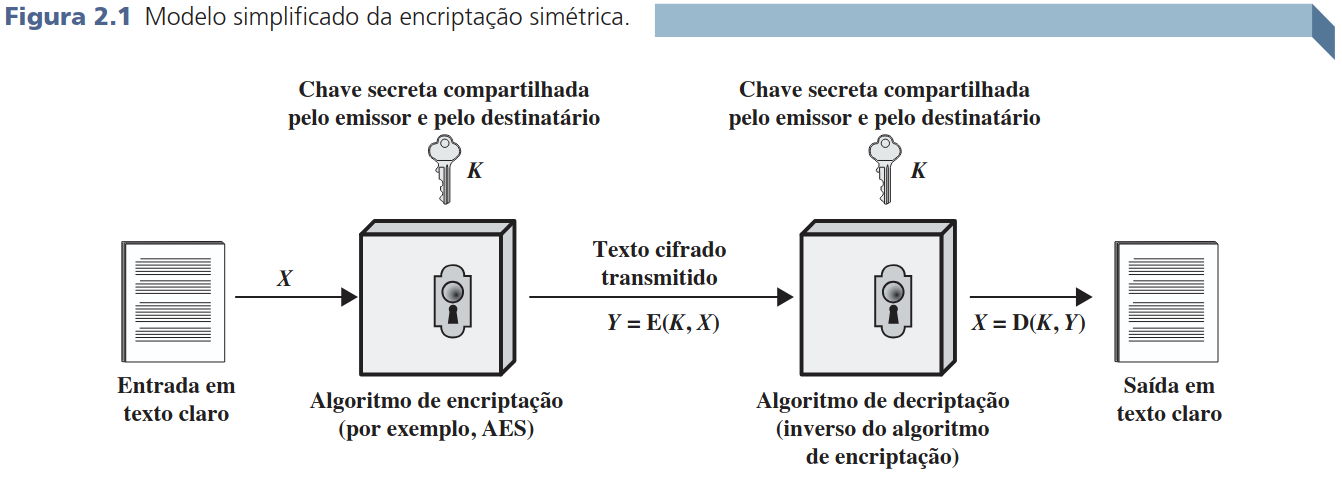
\includegraphics[width=\linewidth]{Figuras/modelo-cripto-simetrica.png}

    \vspace{0.3cm}
    \textbf{Fluxo:} Texto Claro $\xrightarrow{\text{Encriptação + Chave}}$ Texto Cifrado $\xrightarrow{\text{Decriptação + Chave}}$ Texto Claro
\end{frame}

\begin{frame}{Requisitos para o Uso Seguro da Encriptação Simétrica}
    Para que a encriptação simétrica seja efetiva, dois requisitos fundamentais devem ser atendidos:

    \begin{enumerate}
        \item \textbf{Algoritmo forte:} mesmo conhecendo o algoritmo e tendo acesso a textos cifrados (com ou sem os respectivos textos claros), um oponente não deve ser capaz de descobrir a chave ou recuperar o texto claro.
        \item \textbf{Chave protegida:} emissor e receptor devem compartilhar a chave secreta de forma segura e mantê-la em sigilo. Caso a chave seja comprometida, toda a comunicação associada poderá ser lida.
    \end{enumerate}
\end{frame}

\begin{frame}{Segurança na Encriptação Simétrica}
    \begin{itemize}
        \item É impraticável decriptar uma mensagem apenas com o texto cifrado e o conhecimento do algoritmo.
        \item O segredo deve estar somente na \textbf{chave}, não no algoritmo.
        \item Essa característica torna a encriptação simétrica viável para uso generalizado.
        \item Como o algoritmo pode ser público, fabricantes desenvolvem \textbf{chips de baixo custo} com encriptação embutida, hoje comuns em diversos produtos.
        \item Portanto, o principal desafio de segurança é \textbf{manter o sigilo da chave}.
    \end{itemize}
\end{frame}

\begin{frame}{Esquema de Encriptação Simétrica}
    \begin{itemize}
        \item Texto claro: $X = [X_1, X_2, \ldots, X_M]$
        \item Chave de encriptação: $K = [K_1, K_2, \ldots, K_J]$
        \item Texto cifrado: $Y = E(K, X)$
        \item Decriptação: $X = D(K, Y)$
        \item A chave $K$ deve ser compartilhada com segurança entre origem e destino (diretamente ou por terceiro confiável).
    \end{itemize}


    \begin{block}{Visão do Oponente}
        \begin{itemize}
            \item Oponente observa $Y$, mas não conhece $K$.
            \item Supõe-se que conhece os algoritmos $E$ e $D$.
            \item Dois objetivos possíveis:
                  \begin{itemize}
                      \item Recuperar o texto claro $X$, obtendo uma estimativa $\hat{X}$.
                      \item Recuperar a chave $K$, obtendo uma estimativa $\hat{K}$ e assim ler mensagens futuras.
                  \end{itemize}
        \end{itemize}
    \end{block}
\end{frame}


\begin{frame}{Modelo de criptossistema simétrico}
    \centering
    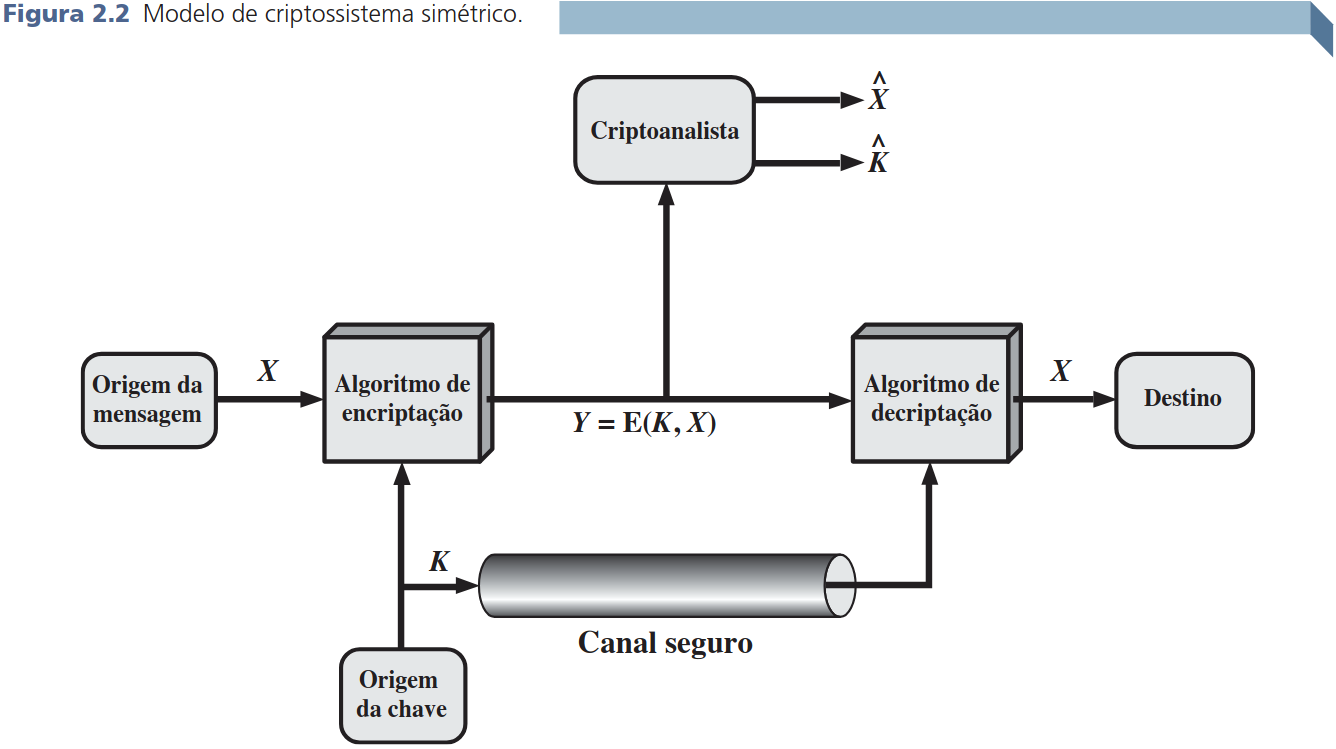
\includegraphics[width=0.9\linewidth]{Figuras/modelo-cripto-simetrico-2.png}


\end{frame}

\begin{frame}{Criptoanálise e Ataque por Força Bruta}
    O objetivo de um ataque é \textbf{recuperar a chave em uso}, não apenas o texto claro.

    \begin{block}{Criptoanálise}
        \begin{itemize}
            \item Explora a natureza do algoritmo de encriptação.
            \item Pode usar conhecimento prévio sobre o texto claro ou pares texto claro–cifrado.
            \item Busca deduzir a chave ou recuperar mensagens específicas.
        \end{itemize}
    \end{block}

    \begin{block}{Ataque por Força Bruta}
        \begin{itemize}
            \item Testa todas as chaves possíveis no texto cifrado.
            \item Em média, é necessário tentar metade do espaço de chaves.
            \item Garante sucesso se houver tempo e poder computacional suficiente.
        \end{itemize}
    \end{block}
\end{frame}

\begin{frame}{Os tipos de Ataques à criptografia}
    A forma de atacar depende da \textbf{quantidade de informação disponível} para o atacante:

    \begin{itemize}
        \item \textbf{Apenas texto cifrado}: cenário mais difícil, exige análise estatística.
        \item \textbf{Algoritmo conhecido}: normalmente se assume que o adversário sabe qual cifra está sendo usada.
        \item \textbf{Ataque por força bruta}: testar todas as chaves possíveis.
              \begin{itemize}
                  \item Impraticável se o espaço de chaves for muito grande.
              \end{itemize}
        \item \textbf{Conhecimento do tipo de texto claro}: facilita a análise (ex.: textos em inglês/francês, arquivos EXE, código fonte, planilhas contábeis).
    \end{itemize}
\end{frame}


\begin{frame}{Ataque de Texto Claro Conhecido }
    O ataque apenas com texto cifrado é o mais fácil de ser defendido, pois o oponente tem a quantidade mínima de informação para trabalhar

    \textbf{Caso:} O atacante possui uma ou mais mensagens em \textbf{texto claro} e suas correspondentes mensagens cifradas.
    \begin{itemize}
        \item Ele pode explorar padrões previsíveis no texto claro.
              \begin{itemize}
                  \item Arquivos com cabeçalhos fixos (ex. PDFs ou logs).
                  \item Mensagens financeiras ou contratos eletrônicos com banners ou formatos padronizados.
                  \item Protocolos de rede com campos fixos (ex.: pacotes com cabeçalhos conhecidos).
              \end{itemize}
        \item Com essas informações, é possível \textbf{deduzir a chave} ou reduzir significativamente o espaço de chaves a ser testado.
        \item Normalmente, ataques de texto claro conhecido são mais efetivos contra cifras fracas ou mal projetadas.
    \end{itemize}

\end{frame}

\begin{frame}{Ataque de Palavra Provável e Texto Claro Escolhido}
    \textbf{Ataque de Palavra Provável:}
    \begin{itemize}
        \item Variante do ataque de texto claro conhecido.
        \item O atacante possui conhecimento parcial de partes da mensagem ou de palavras específicas.
        \item Exemplos:
              \begin{itemize}
                  \item Arquivos de contabilidade com cabeçalhos padronizados ou palavras-chave em posições fixas.
                  \item Código fonte com notas de direitos autorais em posições específicas.
              \end{itemize}
        \item Permite ao atacante reduzir o espaço de chaves a testar ou deduzir padrões na cifra.
    \end{itemize}

    \textbf{Ataque de Texto Claro Escolhido:}
    \begin{itemize}
        \item O atacante consegue que a origem encripte mensagens de sua escolha.
        \item Pode introduzir padrões específicos que ajudem a revelar a estrutura da chave.

    \end{itemize}
\end{frame}

\begin{frame}{Segurança Prática}

    \begin{itemize}
        \item Baseia-se em limitações computacionais ou econômicas do atacante.
        \item Dois critérios principais:
              \begin{itemize}
                  \item \textbf{Custo}: quebrar a cifra é mais caro que o valor da informação.
                  \item \textbf{Tempo}: quebrar a cifra leva mais tempo do que a vida útil da informação.
              \end{itemize}
        \item Objetivo: tornar a decifração inviável na prática, mesmo que teoricamente possível.

        \item Um esquema de encriptação é considerado computacionalmente seguro se um desses dois critérios for atendido.
              \begin{itemize}
                  \item \textbf{Problema}: é muito difícil estimar a quantidade de esforço exigido para criptoanalisar textos
                        cifrados com sucesso.
              \end{itemize}
        \item Ciptoanálise para esquemas de encriptação simétricos são projetadas para explorar o
              fato de que rastros da estrutura ou do padrão do texto claro podem sobreviver à encriptação e ser discerníveis
              no texto cifrado
    \end{itemize}
\end{frame}

\begin{frame}{Cifra de César}
    \textbf{Definição:}
    Uma cifra de substituição simples usada por Júlio César. Cada letra do alfabeto é substituída por aquela que está \textbf{três posições à frente}.

    \medskip
    \textbf{Exemplo:}
    \begin{itemize}
        \item Texto claro: \texttt{meet me after the toga party}
        \item Texto cifrado: \texttt{PHHW PH DIWHU WKH WRJD SDUWB}
    \end{itemize}

    \textbf{Alfabeto:} \\
    \begin{tabular}{c c c c c c c c c c c c c}
        a & b & c & d & e & f & g & h & i & j & k  & l  & m  \\
        0 & 1 & 2 & 3 & 4 & 5 & 6 & 7 & 8 & 9 & 10 & 11 & 12
    \end{tabular}

    \begin{tabular}{c c c c c c c c c c c c c}
        n  & o  & p  & q  & r  & s  & t  & u  & v  & w  & x  & y  & z  \\
        13 & 14 & 15 & 16 & 17 & 18 & 19 & 20 & 21 & 22 & 23 & 24 & 25
    \end{tabular}

    \medskip
    \textbf{Observação:}
    O alfabeto é circular, ou seja, após Z, volta-se para A.
\end{frame}

\begin{frame}{Tabela cifra de César}
    \centering
    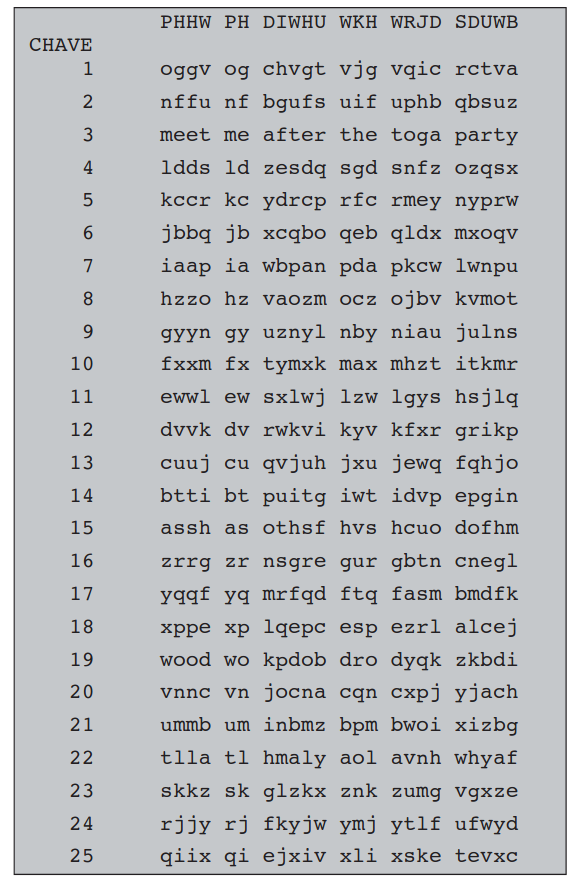
\includegraphics[width=0.35\linewidth]{Figuras/tabela-cifra-cesar.png}


\end{frame}

\begin{frame}{Algoritmo Matemático da Cifra de César}
    \textbf{Cifra de César com deslocamento fixo (3 posições):}
    \[
        C = E(3, p) = (p + 3) \mod 26
    \]

    \textbf{Cifra de César geral com deslocamento \(k\):}
    \[
        C = E(k, p) = (p + k) \mod 26, \quad k \in \{1, 2, \dots, 25\}
    \]

    \textbf{Decifragem:}
    \[
        p = D(k, C) = (C - k) \mod 26
    \]

    \medskip
    \textbf{Observações:}
    \begin{itemize}
        \item Cada letra do alfabeto é mapeada numericamente de 0 a 25.
        \item O operador \(\mod 26\) garante que o alfabeto seja circular (após Z vem A).
        \item Qualquer deslocamento \(k\) no intervalo de 1 a 25 gera uma cifra válida.
        \item \(p\) representa cada letra do texto claro.
    \end{itemize}
\end{frame}

\begin{frame}{Exemplo de Ataque por Palavra Provável - Cifra de César (k=6)}

    \textbf{Texto cifrado:}
    \begin{quote}
        G sotng igyg k asg igyg wak loig vkxzu jk uazxg igyg
    \end{quote}

    \textbf{Texto claro  (César, deslocamento $k=6$):}
    \begin{quote}
        A minha casa e uma casa que fica perto de outra casa
    \end{quote}



    \medskip
    \textbf{Observação:}
    A palavra \textbf{"casa"} aparece repetida várias vezes no texto cifrado (\texttt{igyg}).

    \medskip
    \textbf{Ataque por palavra provável:}
    \begin{itemize}
        \item Reconhecemos padrões repetidos (\texttt{igyg}) que correspondem à palavra "casa".
        \item Com isso, podemos deduzir o deslocamento usado ($k=6$).
        \item Após determinar a chave, podemos decifrar o restante do texto.
    \end{itemize}

    \textbf{Conclusão:}
    Mesmo sem conhecer a chave inicialmente, palavras repetidas permitem descobrir o deslocamento da Cifra de César.
\end{frame}

\begin{frame}{Criptoanálise da Cifra de César por Força Bruta}
    \textbf{Situação:}
    Se soubermos que o texto cifrado é uma cifra de César, podemos usar força bruta para descobrir o texto claro.

    \medskip
    \textbf{Estratégia:}
    \begin{itemize}
        \item Testar todas as 25 chaves possíveis (\(k = 1 \dots 25\)).
        \item Observar qual saída produz texto inteligível.
    \end{itemize}

    \medskip
    \textbf{Exemplo:}
    \begin{itemize}
        \item Texto cifrado: \texttt{PHHW PH DIWHU WKH WRJD SDUWB}
        \item Testando todas as chaves, o texto claro correto aparece na terceira tentativa: \texttt{meet me after the toga party}
    \end{itemize}

    \medskip
    \textbf{Condições que tornam a força bruta viável:}
    \begin{enumerate}
        \item Algoritmos de encriptação e decriptação são conhecidos.
        \item Espaço de chaves pequeno (apenas 25).
        \item Linguagem do texto claro conhecida e reconhecível.
    \end{enumerate}
\end{frame}

\begin{frame}{Limitações da Força Bruta em Algoritmos Modernos}
    \textbf{Situação em redes e criptografia moderna:}
    \begin{itemize}
        \item Algoritmos de encriptação geralmente são conhecidos.
        \item O espaço de chaves é enorme, tornando a força bruta impraticável.
              \begin{itemize}
                  \item Exemplo: Triple DES com chave de 168 bits → \(2^{168} \approx 3,7 \times 10^{50}\) chaves possíveis.
              \end{itemize}
        \item Reconhecimento do texto claro pode ser difícil se:
              \begin{itemize}
                  \item A linguagem do texto não for conhecida.
                  \item O arquivo estiver compactado ou abreviado (ex.: ZIP).
              \end{itemize}
    \end{itemize}

    \textbf{Conclusão:}
    A força bruta é viável apenas em cifras com pequeno espaço de chaves ou quando o texto claro é facilmente reconhecível, como na Cifra de César.
\end{frame}


\begin{frame}{Cifras Monoalfabéticas}
    \textbf{Definição:}
    Uma cifra monoalfabética usa uma permutação completa do alfabeto como chave. Cada letra do texto claro é substituída por uma letra correspondente no alfabeto cifrado.

    \medskip
    \textbf{Exemplo:}

    \begin{tabular}{c|c}
        \textbf{Texto claro} & A B C D E F G H I J K L M N O P Q R S T U V W X Y Z \\
        \textbf{Chave}       & Q W E R T Y U I O P A S D F G H J K L Z X C V B N M \\
    \end{tabular}

    \medskip
    \textbf{Observações:}
    \begin{itemize}
        \item A tabela de substituição (linha do texto cifrado) é a \textbf{chave} do sistema.
        \item Espaço de chave enorme: $26! \approx 4 \times 10^{26}$ possibilidades.
        \item Muito mais seguro que a cifra de César contra ataques por força bruta.
        \item Cada letra do texto claro mapeia para exatamente uma letra do texto cifrado.
    \end{itemize}

    \textbf{Conclusão:}
    Em cifras monoalfabéticas, a chave é a própria permutação do alfabeto, garantindo um espaço de chave muito grande e maior resistência a ataques simples.
\end{frame}

\begin{frame}{Resumo da Lógica das Cifras Monoalfabéticas e César}
    \textbf{O que é público:} O algoritmo, ou seja, como a substituição é feita.
    \textbf{O que é secreto:} A chave, que determina o mapeamento específico.

    \medskip
    \small
    \begin{tabular}{l|c|c}
        \textbf{Característica} & \textbf{Cifra de César}       & \textbf{Substituição Monoalfabética}     \\
        \hline
        Algoritmo               & Substituir por deslocamento   & Substituir por consulta a tabela         \\
        Chave                   & Número $K$ (ex: 3)            & Tabela completa (ex: A→X, B→M, C→O, ...) \\
        Espaço de chaves        & Pequeno (25 chaves possíveis) & Enorme ($26! \approx 4 \times 10^{26}$)  \\
    \end{tabular}

    \medskip
    \textbf{Observação:}
    A segurança de ambos depende do segredo da chave. Enquanto a Cifra de César é vulnerável à força bruta, a cifra monoalfabética é muito mais resistente, \textbf{mas ainda suscetível a ataques de análise de frequência}.
\end{frame}


\begin{frame}{O problema das cifras monoalfabéticas: a frequência das letras}
    \centering
    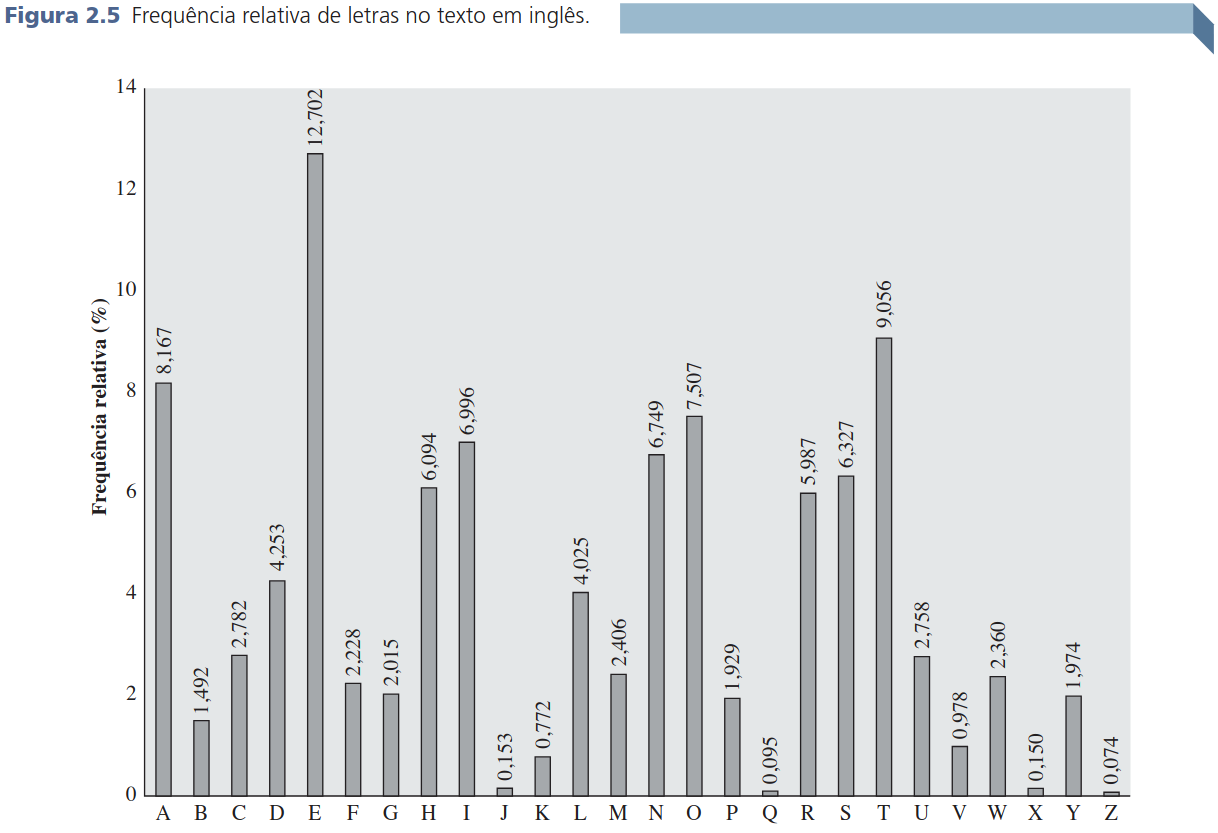
\includegraphics[width=0.8\linewidth]{Figuras/frequencia-letras-ingles.png}


\end{frame}

\begin{frame}{Cifras Monoalfabéticas com Homófonos}
    \textbf{Problema das cifras monoalfabéticas:}
    \begin{itemize}
        \item Frequências de letras do alfabeto original permanecem no texto cifrado.
        \item Isso facilita ataques de análise de frequência.
    \end{itemize}

    \medskip
    \textbf{Solução: Homófonos}
    \begin{itemize}
        \item Atribuir vários símbolos diferentes para a mesma letra do texto claro.
        \item Exemplo: a letra \texttt{E} poderia ser codificada como 16, 74, 35 ou 21, usados aleatoriamente ou em rodízio.
        \item Se o número de homófonos for proporcional à frequência da letra, a informação de frequência única é praticamente eliminada.
    \end{itemize}

    \medskip
    \textbf{Observações:}
    \begin{itemize}
        \item Gauss acreditava ter criado uma cifra indecifrável usando homófonos.
        \item Mesmo com homófonos, padrões de múltiplas letras (digramas, trigramas) ainda podem ser explorados na criptoanálise.
        \item Portanto, ataques baseados em análise estatística ainda são possíveis.
    \end{itemize}
\end{frame}

\begin{frame}{Importância dos Digramas na Criptoanálise}
    \textbf{Por que digramas importam?}
    \begin{itemize}
        \item Análise de digramas detecta \textbf{pares de letras} que aparecem frequentemente em um idioma.
        \item Mesmo cifras monoalfabéticas com homófonos ainda deixam padrões de digramas visíveis.
        \item Cada idioma possui digramas e trigramas comuns; explorá-los ajuda a quebrar cifras.
    \end{itemize}

    \medskip
    \textbf{Exemplos de digramas comuns em português:} DE, ES, EN, NT, RE, RA, AR, OS, TE, CO

    \medskip
    \textbf{Exemplo prático:}
    \begin{itemize}
        \item Texto cifrado com substituição monoalfabética: símbolos \%, \&, \$\# aparecem com frequência.
        \item Suspeita: \% = E, \& = A.
        \item Sequências \%\& e \&\% reforçam os digramas EA e AE.
        \item Sequência \$\#\% sugere "NTE", como em "mente", "gente", "frente".
        \item Padrões de digramas ajudam a deduzir a correspondência de símbolos e letras.
    \end{itemize}



\end{frame}

\begin{frame}{Cifra Playfair}
    \textbf{Características principais:}
    \begin{itemize}
        \item Cifra de múltiplas letras (substitui digramas, não letras isoladas).
        \item Cada par de letras no texto claro é convertido em um digrama no texto cifrado.
        \item Baseada em uma matriz 5×5 de letras.
    \end{itemize}

    \medskip
    \textbf{Construção da matriz:}
    \begin{itemize}
        \item Preencher a matriz com as letras da palavra-chave (sem duplicatas) da esquerda para a direita e de cima para baixo.
        \item Completar a matriz com as letras restantes do alfabeto.
        \item As letras I e J são consideradas uma só.
    \end{itemize}

    \medskip
    \textbf{Resumo do funcionamento:}
    \begin{itemize}
        \item O texto claro é dividido em digramas (pares de letras).
        \item Cada digrama é substituído por outro digrama segundo regras da matriz.
        \item Essa abordagem dificulta a análise por frequência de letras individuais.
    \end{itemize}
\end{frame}

\begin{frame}{Cifra playfair - Chave "monarchy"}
    \centering
    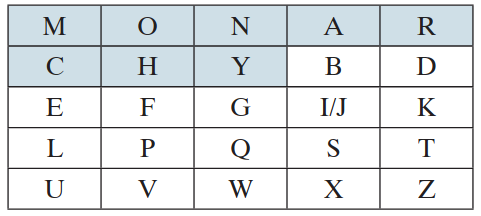
\includegraphics[width=0.8\linewidth]{Figuras/Cifra-playfair.png}


\end{frame}

\begin{frame}{Cifra Playfair - Regras de Encriptação}
    \textbf{Criptografia por digramas:} O texto claro é encriptado duas letras de cada vez.

    \medskip
    \textbf{Regras:}
    \begin{enumerate}
        \item \textbf{Letras repetidas em um par:} Inserir uma letra de preenchimento (ex.: 'x').
              Exemplo: \texttt{balloon} $\rightarrow$ \texttt{ba lx lo on}.

        \item \textbf{Letras na mesma linha da matriz:} Substituir cada letra pela à direita, de forma rotativa.
              Exemplo: \texttt{ar} $\rightarrow$ \texttt{RM}.

        \item \textbf{Letras na mesma coluna da matriz:} Substituir cada letra pela abaixo, de forma rotativa.
              Exemplo: \texttt{mu} $\rightarrow$ \texttt{CM}.

        \item \textbf{Caso geral (retângulo):} Cada letra do par é substituída pela letra na sua linha e na coluna da outra letra do par.
              Exemplo: \texttt{hs} $\rightarrow$ \texttt{BP}, \texttt{ea} $\rightarrow$ \texttt{IM} (ou JM).
    \end{enumerate}
\end{frame}

\begin{frame}{Cifra Playfair - Contexto e Segurança}
    \textbf{Avanços sobre cifras monoalfabéticas:}
    \begin{itemize}
        \item Enquanto uma cifra monoalfabética lida com 26 letras, a Playfair trabalha com 26 × 26 = 676 digramas.
        \item A análise de frequência torna-se muito mais difícil, pois os padrões de digramas são menos evidentes.
        \item Foi considerada indecifrável por muito tempo.
    \end{itemize}

    \textbf{Uso histórico:}
    \begin{itemize}
        \item Sistema de campo padrão do Exército britânico na Primeira Guerra Mundial.
        \item Ainda usada pelo Exército dos EUA e forças aliadas na Segunda Guerra Mundial.
    \end{itemize}

    \textbf{Limitações:}
    \begin{itemize}
        \item Apesar da aparente segurança, a Playfair ainda deixa rastros da estrutura da linguagem do texto claro.
        \item Algumas centenas de letras de texto cifrado geralmente são suficientes para quebrá-la.
    \end{itemize}
\end{frame}


\begin{frame}{Cifras Polialfabéticas e Vigenère}
    \textbf{Cifras polialfabéticas:}
    \begin{itemize}
        \item Melhoram as cifras monoalfabéticas usando diferentes substituições ao longo da mensagem.
        \item Um conjunto de regras de substituição monoalfabéticas é utilizado.
        \item Uma chave define qual regra é aplicada a cada posição da mensagem.
    \end{itemize}

    \textbf{Cifra de Vigenère:}
    \begin{itemize}
        \item Uma das mais conhecidas e simples cifras polialfabéticas.
        \item Utiliza 26 cifras de César com deslocamentos de 0 a 25.
        \item Texto cifrado $C = C_0, C_1, ..., C_{n-1}$ é calculado como:
              \[
                  C_i = (p_i + k_j) \mod 26
              \]
              onde $p_i$ é a letra do texto claro e $k_j$ é a letra da chave, repetindo a chave conforme necessário.
    \end{itemize}

    \textbf{Resumo:}
    Cada letra do texto claro é cifrada usando uma regra que varia ao longo da mensagem, definida pela chave.
\end{frame}

\begin{frame}{Cifra de Vigenère: Operação Detalhada}
    \textbf{Como funciona:}
    \begin{itemize}
        \item Cada letra do texto claro é cifrada usando uma letra da chave correspondente.
        \item Para textos mais longos que a chave, a chave é repetida ciclicamente.
    \end{itemize}

    \textbf{Equação de encriptação:}
    \[
        C_i = (p_i + k_{i \mod m}) \mod 26
    \]
    \begin{itemize}
        \item $p_i$: letra do texto claro na posição $i$
        \item $k_{i \mod m}$: letra da chave correspondente, repetida quando necessário
        \item $m$: comprimento da chave
    \end{itemize}

    \textbf{Equação de decriptação:}
    \[
        p_i = (C_i - k_{i \mod m}) \mod 26
    \]

    \textbf{Comparação com César:}
    Cada caractere do texto claro é cifrado com uma cifra de César diferente, determinada pela letra da chave.

\end{frame}

\begin{frame}{Cifra de Vigenère - Exemplo}
    \begin{itemize}
        \item \textbf{Palavra-chave}: "deceptive"
        \item \textbf{Mensagem}: "we are discovered save yourself"
    \end{itemize}
    \vspace{0.5cm}
    \centering
    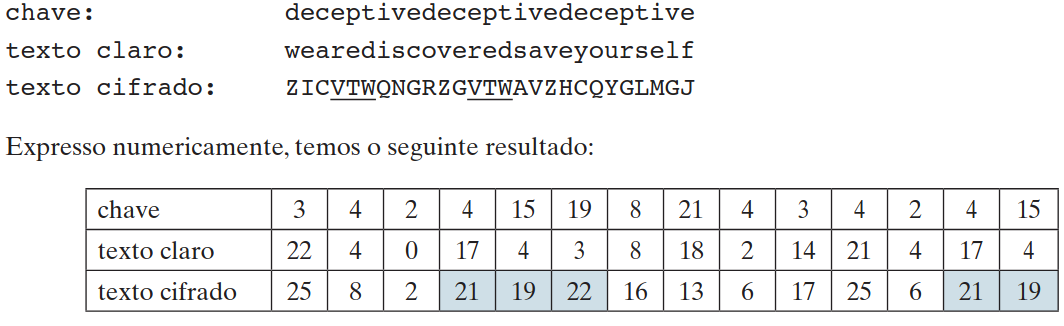
\includegraphics[width=\linewidth]{Figuras/Exemplo-Cifra-de-Vigenere.png}



\end{frame}

\begin{frame}{Vulnerabilidade da Cifra de Vigenère}
    \textbf{Ocultação da frequência de letras:}
    Cada letra do texto claro pode gerar múltiplas letras cifradas, dependendo da letra correspondente da chave, dificultando a análise de frequência simples.

    \medskip
    \textbf{Informações ainda presentes:}
    Apesar da melhoria em relação à cifra Playfair, padrões do texto claro ainda podem aparecer. Por exemplo, sequências repetidas no texto cifrado podem indicar o comprimento da chave.

    \medskip
    \textbf{Exemplo:}
    Um analista observa que a sequência ``VTW'' aparece duas vezes a uma distância de 9 caracteres.
    Isso sugere que a chave pode ter 3 ou 9 letras de extensão, embora a repetição possa ser casual.

    \medskip
    \textbf{Ataque possível:}
    Se a mensagem for longa, múltiplas sequências repetidas permitem ao analista estimar o tamanho da chave.
    Esse é o princípio do ataque de Kasiski, usado para quebrar cifras polialfabéticas.
\end{frame}

\begin{frame}{Cifra de Vigenère com Auto-Chave}
    \textbf{Problema da repetição da chave:}
    A periodicidade da palavra-chave facilita ataques de criptoanálise.

    \medskip
    \textbf{Solução proposta por Vigenère:}
    Usar uma palavra-chave concatenada ao próprio texto claro, formando uma \textit{chave corrente} tão longa quanto a mensagem.

    \medskip
    \textbf{Exemplo:}
    \begin{itemize}
        \item Chave: \texttt{deceptivewearediscoveredsav}
        \item Texto claro: \texttt{wearediscoveredsaveyourself}
        \item Texto cifrado: \texttt{ZICVTWQNGKZEIIGASXSTSLVVWLA}
    \end{itemize}

    \medskip
    \textbf{Observação:}
    Mesmo assim, o esquema ainda é vulnerável à criptoanálise estatística, pois a chave compartilha a distribuição de frequência do texto claro.
\end{frame}



\begin{frame}{Cifra de Vernam}
    \textbf{Ideia principal:}
    Usar uma palavra-chave tão longa quanto o texto claro, sem relação estatística com ele.

    \medskip
    \textbf{Introdução:}
    Proposta em 1918 por \textit{Gilbert Vernam}, engenheiro da AT\&T.
    Opera sobre \textbf{dados binários} (bits), e não sobre letras.

    \medskip
    \textbf{Definição:}
    \[
        c_i = p_i \oplus k_i
    \]
    \[
        p_i = c_i \oplus k_i
    \]
    onde:
    \begin{itemize}
        \item $p_i$ = bit do texto claro na posição $i$,
        \item $k_i$ = bit da chave na posição $i$,
        \item $c_i$ = bit do texto cifrado na posição $i$,
        \item $\oplus$ = operação \textit{XOR} (OU-exclusivo).
    \end{itemize}

    \medskip
    \textbf{Observação:}
    Vernam propôs uma chave muito longa, mas ainda repetida.
    Com texto cifrado suficiente, o sistema pode ser quebrado com análise estatística e \textit{texto claro provável}.
\end{frame}

\begin{frame}{Cifra de Vernam}


    \centering
    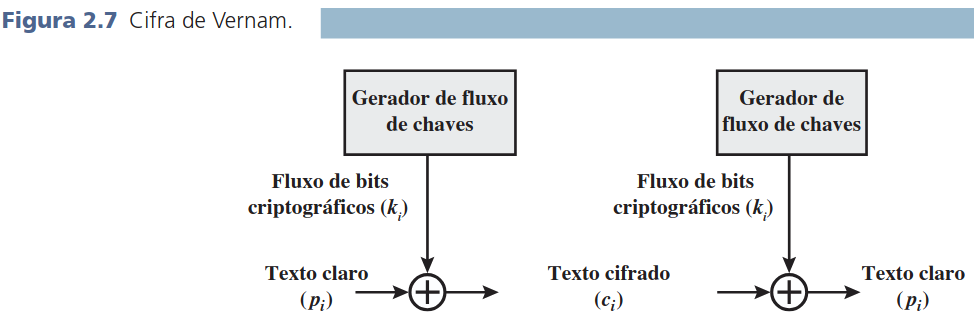
\includegraphics[width=\linewidth]{Figuras/cifra-de-vernam.png}



\end{frame}


\begin{frame}{One-Time Pad}
    \textbf{Melhoria proposta por Joseph Mauborgne (Exército dos EUA):}
    \begin{itemize}
        \item Uso de uma \textbf{chave aleatória}, tão longa quanto a mensagem.
        \item A chave nunca é repetida.
        \item Cada mensagem exige uma nova chave, que deve ser descartada após o uso.
    \end{itemize}

    \medskip
    \textbf{Propriedades:}
    \begin{itemize}
        \item O texto cifrado é totalmente aleatório.
        \item Não existe correlação estatística com o texto claro.
        \item \textbf{Inquebrável}: não há informação no texto cifrado que permita deduzir o texto claro sem a chave.
    \end{itemize}

\end{frame}

\begin{frame}{Exemplo - One-time pad}


    \centering
    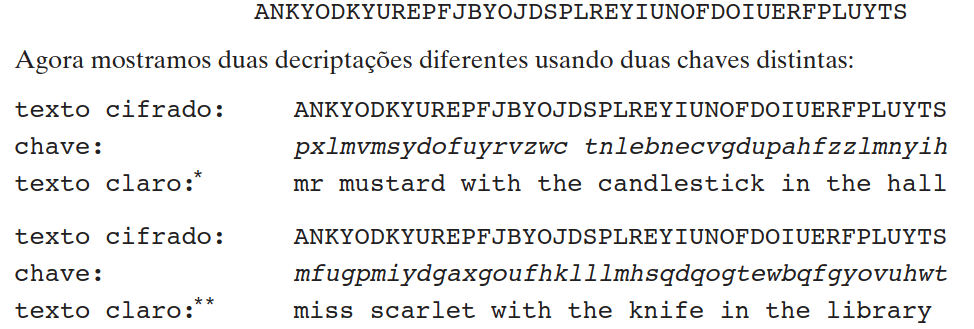
\includegraphics[width=\linewidth]{Figuras/exemplo-one-time-pad.png}



\end{frame}

\begin{frame}{One-Time Pad: Segurança e Limitações}
    \textbf{Segurança:}
    \begin{itemize}
        \item A segurança decorre inteiramente da \textbf{aleatoriedade da chave}.
        \item Se a chave é verdadeiramente aleatória, o texto cifrado também será.
        \item Não existem padrões ou regularidades para um criptoanalista explorar.
        \item Representa a \textbf{cifra perfeita}: segurança completa em teoria.
    \end{itemize}

    \medskip
    \textbf{Limitações práticas:}
    \begin{enumerate}
        \item Geração de grandes quantidades de números verdadeiramente aleatórios.
        \item Distribuição e proteção das chaves — uma nova chave, do mesmo tamanho da mensagem, é necessária para cada comunicação.
    \end{enumerate}

    \begin{block}{Segredo perfeito}
        Por causa dessas dificuldades, o one-time pad tem utilidade limitada, e aplicação principalmente para canais
        de pouca largura de banda que exigem segurança muito alta.
        O one-time pad é o único criptossistema que apresenta o que é conhecido como \textbf{segredo perfeito}.
    \end{block}
\end{frame}


